\section{Introduction}

To be able to execute currently known useful quantum algorithms, a computer with near-perfect qubits and gates is needed.
As individual qubits and gates are far from perfect,
the plan is to employ \emph{quantum error correction} (QEC) to build a fault-tolerant quantum computer.
A quantum computing scheme is considered fault-tolerant if its output is correct with high probability, even though its individual components are faulty.
A popular strategy for implementing fault-tolerant quantum computing is to perform gates through lattice surgery on qubits encoded in the surface code \cite{dennis2002topological,Horsman_2012_lattice_surgery,Litinski2019gameofsurfacecodes, gidney2021factor}.
The basic unit of a lattice surgery computer is a single qubit encoded in the surface code for a fixed unit of time. 
We refer to this unit as a  \textit{surface code block}.
It is an exciting time for lattice surgery computing, with several experimental prototypes of surface code blocks demonstrated 
\cite{acharya2024quantum, caune2024demonstrating, wootton2022measurements, eickbusch2024demonstrating, ali2024reducing, krinner2022realizing, harper2025characterising}.


In parallel with the development of these prototypes, the recent discovery of \textit{dynamic stabilizer codes} has led to new ways of implementing surface code blocks. This started with the introduction of the Hastings-Haah honeycomb code \cite{hastings2021dynamically}.
Subsequently, a larger class of codes containing the honeycomb code was discovered, which we refer to as \textit{dynamically condensed colour codes} (DCCCs) \cite{kesselring2022anyon}.
Despite having `colour code' in their name, DCCCs are topologically equivalent to the surface code, so can be used as surface code blocks
\cite{davydova2022floquet, bombin2024unifying, kesselring2022anyon}. 

Schemes for fault-tolerant quantum computing have an enormous resource cost for implementation with modern technology.
For this reason, the main motivation for looking for new QEC codes is to reduce the resource requirements of a fault-tolerant computer. Importantly, the performance of a QEC code depends on the characteristics of the noise that affects a computer. 
Notably, for many hardware platforms, the noise can be biased towards certain types of operations.
For example, a certain Pauli error ($Z$, say) can be more likely to occur than another ($X$ or $Y$, say).
In the past, it has been shown that QEC codes can be tailored to deal with biased noise
\cite{bonilla2021xzzx, darmawan2021practical, OscarSubsystemGaugeFixing, Miguel2023cellularautomaton, Srivastava2022xyzhexagonal, NonIID, PhysRevLett.133.110601,Tuckett2018,Tuckett2019, Tuckett2020}.
These results have been so promising that some quantum computers are now designed such that the noise is
deliberately biased \cite{darmawan2021practical}.
However, fewer works look at tailoring codes 
to hardware platforms where measurement errors are dominant --
i.e.\ where measurements are more faulty than other types of quantum operations.
This type of biased noise is relevant to multiple hardware proposals based on superconducting qubits~\cite{harper2025characterising, rigetti_qpus, iqm_radiance}.


In this work, we investigate the resource requirements of a lattice surgery quantum computer that uses a DCCC.
Simulations have shown promising results for the \textit{space} cost of two specific DCCCs under an unbiased noise model \cite{gidney2021fault, gidney2022benchmarking, kesselring2022anyon}.
However, the \textit{spacetime} cost provides a more precise measure for resource estimation of a lattice surgery quantum computer. This has not previously been studied for either uniform or biased noise models.
To measure the spacetime cost, we generalise the teraquop footprint~\cite{gidney2021fault} to the \textit{teraquop volume}, defined as the product of the number of qubits and the number of rounds required to achieve a logical error rate of $10^{-12}$, the so-called \textit{teraquop regime}.
A logical error rate of $10^{-12}$ or lower would be required for a lattice surgery quantum computer to be able to solve important problems~\cite{lee2021even, gidney2021factor, haner2020improved,gidney2025factor,bourdoncle2026two}.
% We develop a numerical procedure to find the teraquop volume and carry it out for several biased noise models, including models biased towards measurement noise.

\subsection{Previous numerical work}\label{subsec:previous-numerical-work}

The footprint of what we'll refer to as the $X^1 Y^1 Z^1$ honeycomb code has been studied in \Ccite{gidney2022benchmarking, gidney2021fault, dessertaine2025, chan2025tailoring}.
The footprints of hyperbolic and semi-hyperbolic $X^1 Y^1 Z^1$ honeycomb codes have been studied in \Ccite{higgott2024constructions,sutcliffe2025distributedquantumerrorcorrection}. 
The memory threshold of what we'll refer to as the $X^1 Z^1$ honeycomb code has been studied in \Ccite{kesselring2022anyon, Hetnyi2024}. 
The memory threshold of the $X^1 Z^1$ honeycomb code tailored to biased noise has been studied in \Ccite{setiawan2024tailoring}. 
Measurements of $X^1 Y^1 Z^1$ and $X^1 Z^1$ honeycomb code plaquette stabilizers have been performed on superconducting hardware \cite{wootton2022measurements}.

\subsection{Overview of results}\label{subsec:results}

We simulate a large class of DCCCs which are defined by their \textit{measurement schedules}.
All DCCCs are implemented by repeatedly measuring sets of $XX$, $YY$ or $ZZ$ operators according to certain rules.
Additionally, one can choose to repeat a particular set of weight-two measurements any number of times~\cite{OscarSubsystemGaugeFixing}.
A glossary of the terms used in the figures within this section is provided in Table \ref{tab:glossary}.

\subsubsection{Direct parity measurement noise results}\label{subsubsec:direct-parity-measurement-noise-results}

\Cref{fig:phenomenological_noise_volume_plot_beliefmatching,fig:phenomenological_noise_volume_plot_pymatching} show the performance of DCCCs for direct parity measurement noise models decoded using MWPM and belief matching.
We have obtained volumes for 16 different noise models, which differ in measurement bias and $Z$ error bias.
From the results presented in \Cref{fig:phenomenological_noise_volume_plot_beliefmatching,fig:phenomenological_noise_volume_plot_pymatching}, we can draw the following conclusions:

\begin{keypoint}
When decoding with MWPM, it is better to only measure $XX$ and $ZZ$, while when decoding with belief matching, it is better to measure $XX$, $YY$, and $ZZ$.
\end{keypoint}

\begin{keypoint}
Repeating measurements can improve the teraquop volume under measure\-ment-biased noise.
\end{keypoint}



\subsubsection{Auxiliary qubit circuit noise results}\label{subsubsec:auxiliary-qubit-circuit-noise-results}

Three auxiliary qubit circuit noise models are simulated: \emph{superconducting-inspired} (SI) noise, \emph{standard depolarizing} (SD) noise, and \emph{entangling
measurement} (EM) noise.
\Cref{fig:pymatching_circuit_level_noise_volume_plot,fig:beliefmatching_circuit_level_noise_volume_plot} show the performance of DCCCs when decoded with MWPM and belief matching, respectively. 
We can draw the following conclusions:

\begin{keypoint}
For all three auxiliary qubit circuit noise models, when decoding with MWPM, it is better to only measure $XX$ and $ZZ$, while when decoding with belief matching, it is better to measure $XX$, $YY$, and $ZZ$.
\end{keypoint}

\begin{keypoint}
The noise bias in the SI noise model is not strong enough to make repeating measurements worthwhile.
\end{keypoint}

\begin{keypoint}
For EM noise and decoding using MWPM the best DCCC is $X^2Z^2$.
\end{keypoint}

We consider this a key point because DCCCs are especially well suited for EM noise.
Namely, for this noise model, it has been shown that the teraquop footprint of the $X^1 Y^1 Z^1$ code is smaller than the teraquop footprint of the surface code implemented with pair measurements~\cite{gidney2023pair,paetznick2023performance}.

\subsubsection{Remainder of this work}\label{subsubsec:remainder-of-this-work}

\Cref{sec:DCCCs} contains background information on DCCCs.
If you are familiar with DCCCs, detectors, logical errors, and decoding graphs, you can skip \Cref{sec:DCCCs}.
In \Cref{sec:teraquop_volume} we introduce and explain the teraquop volume, a key performance metric which we use to evaluate the performance of QEC protocols.
The remainder of this work
is dedicated to understanding the main results and explaining how these results have
been obtained.
We first focus on the results comparing the $X^1 Z^1$ and $X^1 Y^1 Z^1$ codes in \Cref{sec:choosing-a-schedule}.
Following this we discuss how and why repeating measurement influences spacetime cost in \Cref{sec:gauge_dcccs}.
We finish this work with a summary and outlook in \Cref{sec:summary_and_outlook}.
The source code used to produce the results in this paper can be found at \\
\url{https://github.com/peter-janderks/floquet_colour_codes_numerics}.

\begin{table}[htbp]
    \renewcommand{\arraystretch}{1.2}
    \scalebox{0.9}{
        \begin{tabularx}{\textwidth}{l|X}
            \hline
    %  \multicolumn{2}{c}%{\textbf{Section \ref{sec:DCCCs}}} \\
            \hline
            \makecell[lt]{$X^a Y^b Z^c$ code \\$a,b,c \in \mathbb{Z}_{>0}$} & DCCC whose measurement schedule consists of $a$ consecutive $XX$ measurements, $b$ consecutive $YY$ measurements, and $c$ consecutive $ZZ$ measurements on certain qubits. \\
            \makecell[lt]{$X^a Z^b$ code\\$a,b,c \in \mathbb{Z}_{>0}$} & DCCC whose measurement schedule consist of $a$ consecutive $XX$ measurements and $b$ consecutive $ZZ$ measurements on certain qubits.\\
            \makecell[lt]{Teraquop\\volume} & The amount of qubits times the number of measurement rounds at which the probability of any logical error occurring is $10^{-12}$.  \\
            MWPM & A decoder that uses the minimum-weight perfect-matching algorithm.\\
            \makecell[lt]{Belief\\matching} &  A decoder that uses belief propagation and the minimum-weight perfect-matching algorithm.\\
            \makecell[lt]{Direct parity\\measurement noise} & A circuit noise model in which single-qubit Pauli errors can occur before measurement rounds with probabilities $p_X$, $p_Y$ and $p_Z$, and measurement errors can occur with probability $p_m$. Assumes native two-qubit parity measurements.\\
            \makecell[lt]{Measurement\\error bias} & $\frac{p_m}{p_X + p_Y + p_Z}$, assuming $p_X, p_Y, p_Z$ and $p_m$ are chosen such that the physical error rate is kept constant at $10^{-3}$.\\
            \makecell[lt]{$Z$ error\\bias} & $\frac{2p_Z}{p_X+p_Y}$, assuming $p_X, p_Y, p_Z$ and $p_m$ are chosen such that the physical error rate is kept constant at $10^{-3}$.\\
            \makecell[lt]{Auxiliary qubit\\circuit noise} & A circuit noise model in which a $q$-qubit Pauli error can occur with probability $p_g$ after each gate $g$ on $q$ qubits, and measurement errors can occur with probability $p_m$. Multi-qubit measurements are decomposed using auxiliary qubits.\\
            \makecell[lt]{Standard\\depolarizing noise} & An auxiliary qubit circuit noise model that assumes multi-qubit measurements are implemented by single-qubit measurements on auxiliary qubits, and all error probabilities are equal.\\
            \makecell[lt]{Superconducting-\\inspired noise} & An auxiliary qubit circuit noise model that assumes multi-qubit measurements are implemented by single-qubit measurements on auxiliary qubits, and the error probabilities model those experienced by real superconducting hardware.\\
            \makecell[lt]{Entangling\\measurement noise} & An auxiliary qubit circuit noise model that assumes multi-qubit measurements are implemented directly, and all error probabilities are equal.\\
            \hline
        \end{tabularx}
    }
    \caption{
        Glossary for terms used in Figs.\  \ref{fig:phenomenological_noise_volume_plot_pymatching}, \ref{fig:phenomenological_noise_volume_plot_beliefmatching}, \ref{fig:pymatching_circuit_level_noise_volume_plot}, and \ref{fig:beliefmatching_circuit_level_noise_volume_plot}.
        More information on the noise models is given in \Cref{subsec:noise_models}.}
    \label{tab:glossary}
\end{table}

\begin{figure}[p]
    \centering
    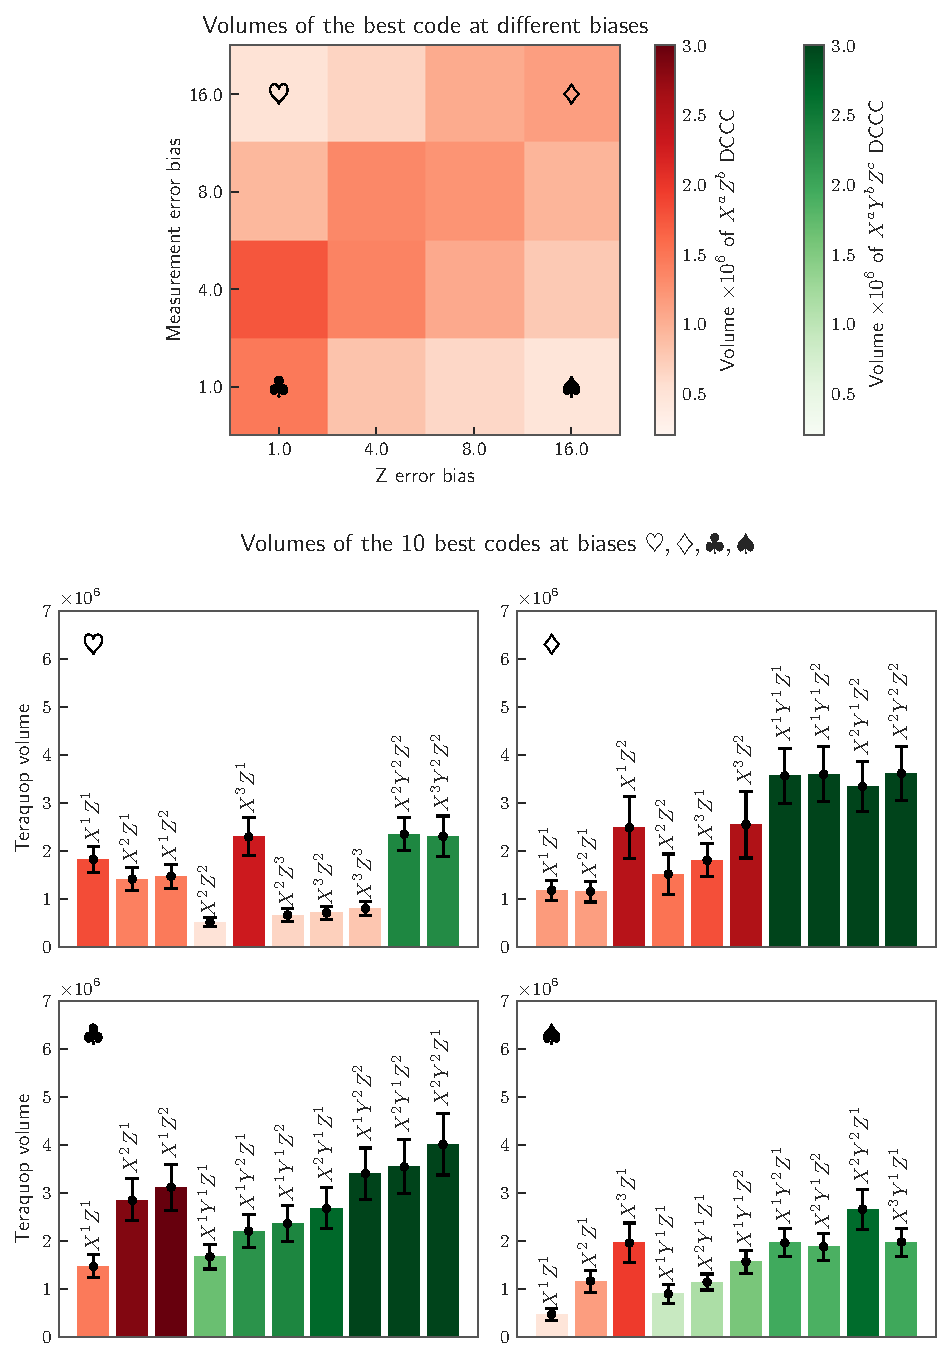
\includegraphics[width=0.9\columnwidth]{figures/introduction/spacetime_volume_heatmap_pymatching.pdf}
    \caption{Squares in the top patchwork plot are red (green) if the code with the smallest teraquop volume is an $X^aZ^b$ code ($X^aZ^bY^c$ code).
        A darker shade indicates a higher volume.
        The four bar plots show the footprints of the 10 best codes at the four limits of the simulated biases.
        The error bars are explained in \Cref{sec:methodology}.
        Decoding is performed using MWPM.
        For all noise models investigated here, the $X^a Z^b$ code outperforms the $X^a Y^b Z^c$ code.
        Repeating measurements improves performance when the noise is biased strongly towards measurement errors only, and has negligible effect otherwise.
        Codes are ordered first by type ($X^a Z^b$ code, then $X^a Y^b Z^c$ code), then by increasing schedule length ($a+b$ or $a+b+c$). 
        Codes with equal schedule length are ordered by balance, with more uniformly distributed repetition parameters appearing first.
        For noise model details, definitions, and naming conventions see Table \ref{tab:glossary}.
     }
    \label{fig:phenomenological_noise_volume_plot_pymatching}
\end{figure}


\begin{figure}[p]
    \centering
    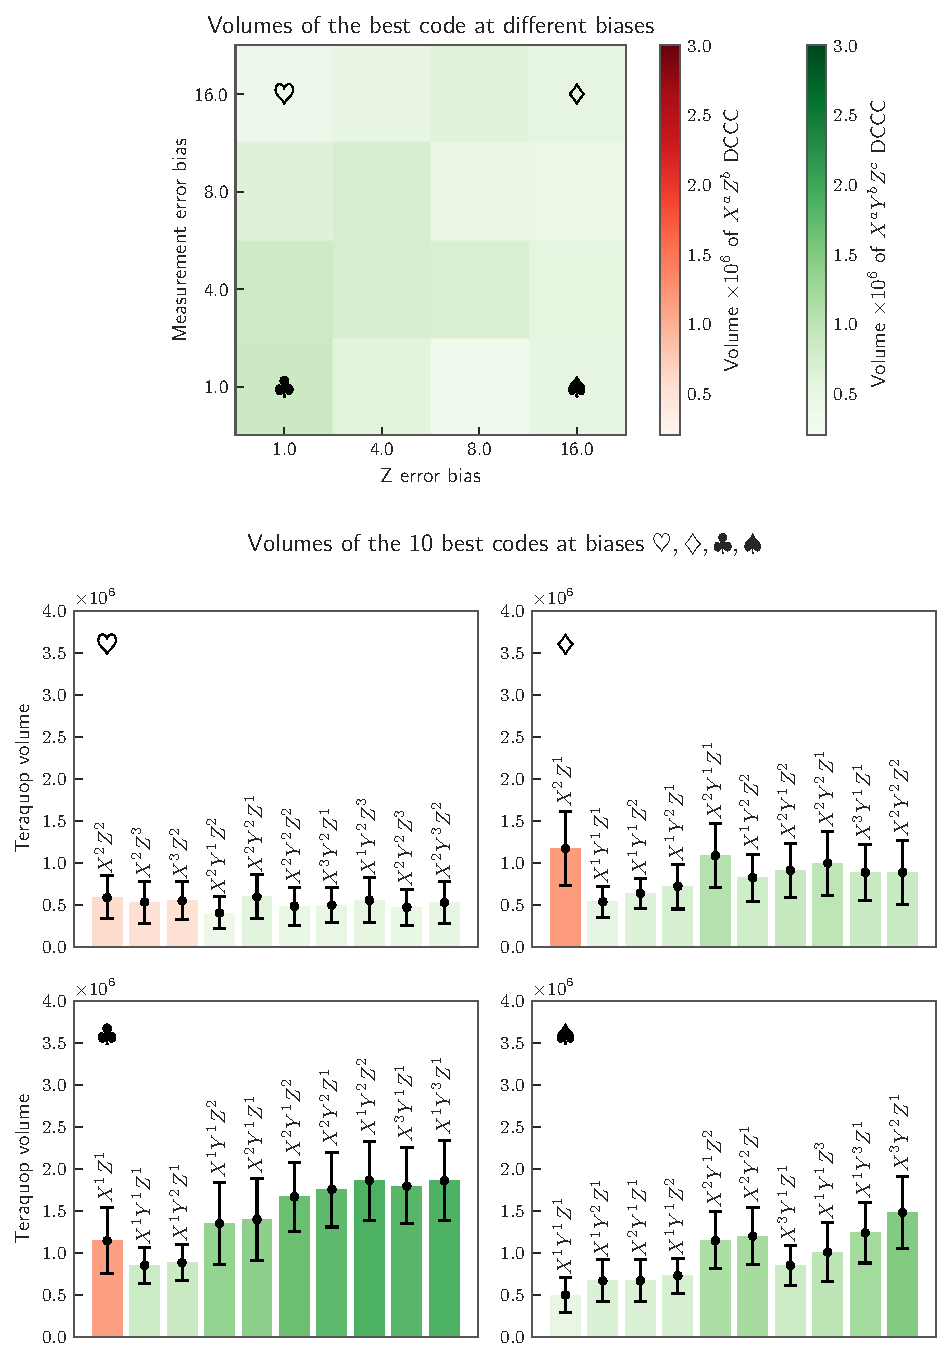
\includegraphics[width=0.9\columnwidth]{figures/introduction/spacetime_volume_heatmap_beliefmatching.pdf}
    \caption{
        Same plot as in \Cref{fig:phenomenological_noise_volume_plot_pymatching} but with decoding performed using belief matching.
        In contrast to \Cref{fig:phenomenological_noise_volume_plot_pymatching}, for all noise models investigated here, the $X^a Y^b Z^c$ code outperforms the $X^a Z^b$ code.
        However, as before, repeating measurements improves performance when the noise is biased strongly towards measurement errors only, but has negligible effect otherwise.
    }
    \label{fig:phenomenological_noise_volume_plot_beliefmatching}
\end{figure}

\begin{figure}[p]
    \centering
    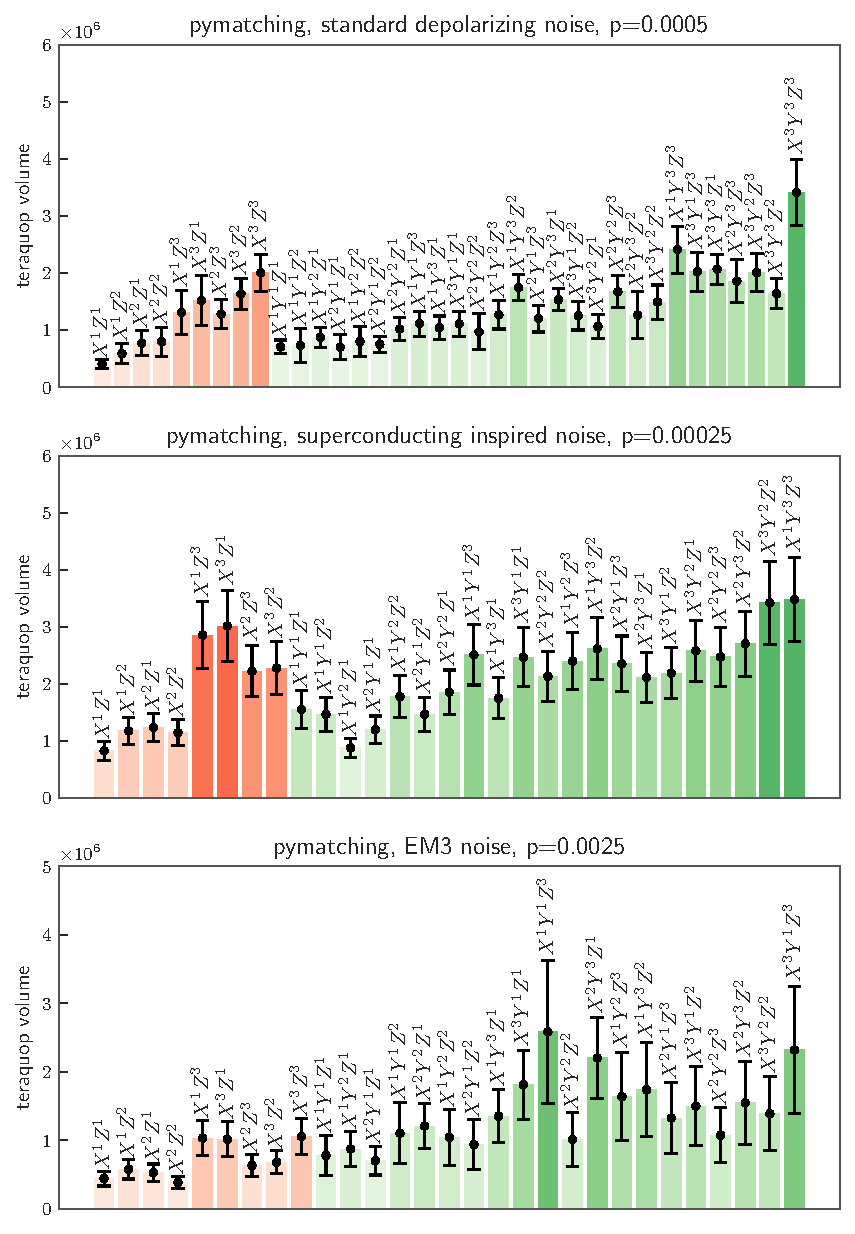
\includegraphics[width=0.9\columnwidth]{figures/introduction/volumes_cln_pymatching.pdf}
    \caption{Teraquop volumes of $X^a Y^b Z^c$ and $X^a Z^b$ codes for three auxiliary qubit circuit noise models; standard depolarizing noise with $p=0.0005$, superconducting inspired noise with $p=0.00025$, and entangling measurement noise with $p=0.0025$. Decoding is performed using MWPM. 
    Codes are ordered first by type ($X^a Z^b$ code, then $X^a Y^b Z^c$ code), then by increasing schedule length ($a + b$ or $a+b+c$). 
    Codes with equal schedule length are ordered by balance, with more uniformly distributed repetition parameters appearing first.
    In each case, the code with the best teraquop volume is from the $X^a Z^b$ family, though the difference is small.
    Repeating measurements broadly has negligible effect, though does seem to improve the performance of the $X^1 Y^1 Z^1$ code in the superconducting inspired noise model, which features a moderate measurement bias.
    The error bars are explained in \Cref{sec:methodology}.}
    \label{fig:pymatching_circuit_level_noise_volume_plot}
\end{figure}

\begin{figure}[p]
    \centering
    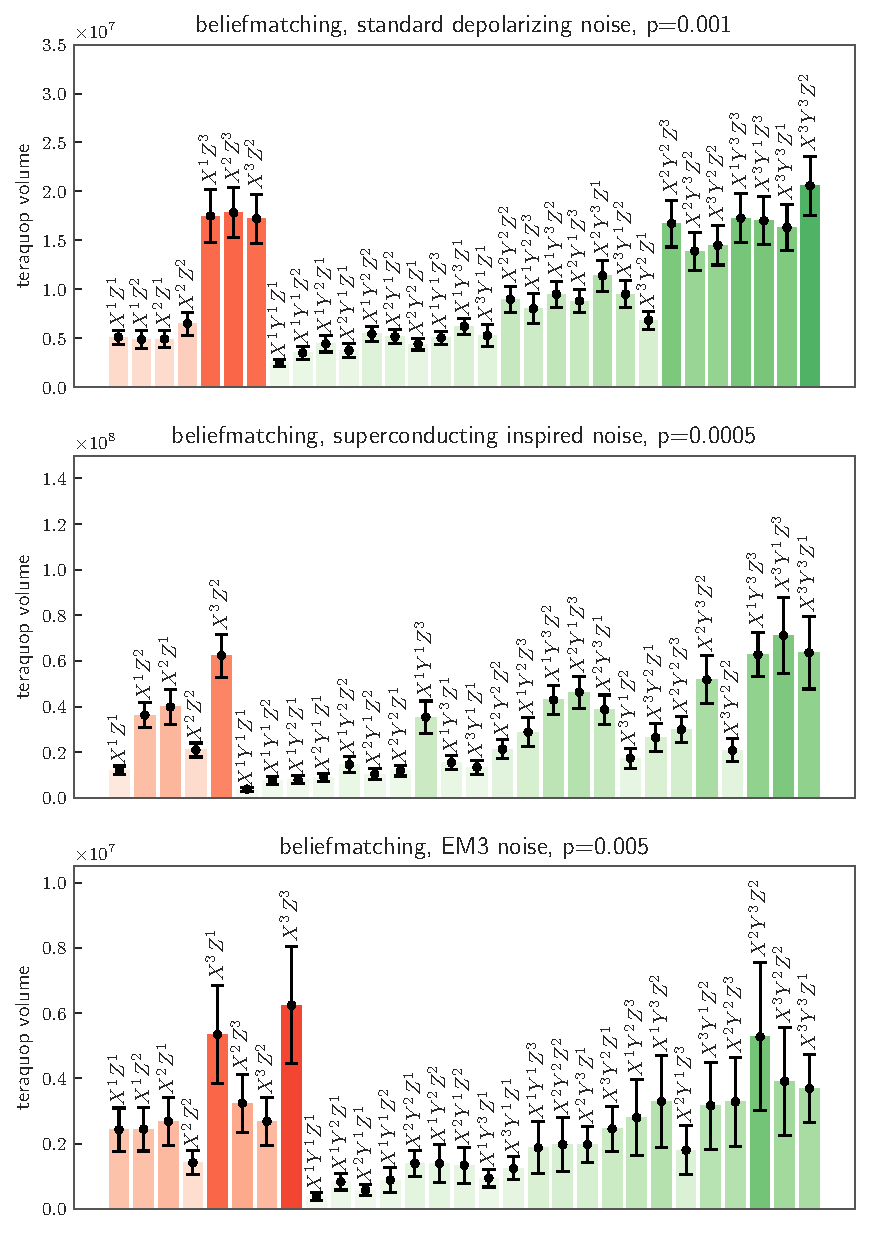
\includegraphics[width=0.9\columnwidth]{figures/introduction/volumes_cln_beliefmatching.pdf}
  \caption{
    Same plot as in \Cref{fig:pymatching_circuit_level_noise_volume_plot} but with decoding performed using belief matching and higher physical error rates;
    standard depolarizing noise with $p=0.001$, superconducting inspired noise with $p=0.0005$, and entangling measurement noise with $p=0.005$. 
    As before, repeating measurements broadly has negligible effect, though does improve the performance of the $X^1 Z^1$ code in the entangling measurements noise model.}
    \label{fig:beliefmatching_circuit_level_noise_volume_plot}
\end{figure}


\FloatBarrier

